% a=3,b=2; u=9/4,v=1. Orthogonal feet are computed exactly.
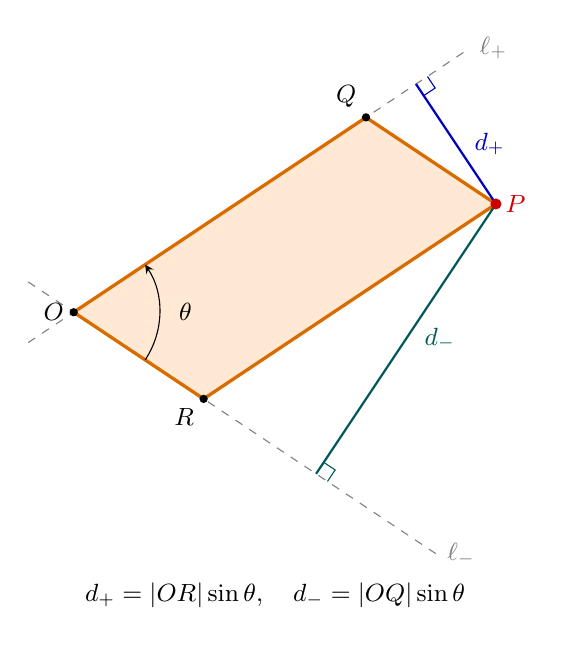
\begin{tikzpicture}[x=1.65cm,y=1.65cm,>=stealth,font=\small]
\coordinate (O) at (0,0); \coordinate (Q) at (2.25,1.5);
\coordinate (R) at (1,-2/3); \coordinate (P) at (3.25,5/6);
\coordinate (A) at (137/52,137/78);
\coordinate (B) at (97/52,-97/78);
\fill[orange!17] (O)--(Q)--(P)--(R)--cycle;
\draw[gray,dashed] (-.35,-7/30)--(3.05,61/30) node[right] {$\ell_+$};
\draw[gray,dashed] (-.35,7/30)--(2.8,-28/15) node[right] {$\ell_-$};
\draw[orange!85!black,very thick] (O)--(Q)--(P)--(R)--cycle;
\draw[blue!75!black,thick] (P)--(A) node[midway,right=3pt] {$d_+$};
\draw[teal!70!black,thick] (P)--(B) node[midway,right=3pt] {$d_-$};
% right angle markers at A and B
\draw[blue!75!black] (2.7231,1.8141)--(2.7819,1.7259)--(2.6937,1.6671);
\draw[teal!70!black] (1.9536,-1.3024)--(2.0124,-1.2142)--(1.9242,-1.1554);
\draw[->] (0.55,-.3667) arc[start angle=-33.6901,end angle=33.6901,radius=.661];
\node at (.86,0) {$\theta$};
\fill (O) circle(1.5pt) node[left] {$O$};
\fill (Q) circle(1.5pt) node[above left] {$Q$};
\fill (R) circle(1.5pt) node[below left] {$R$};
\fill[red!80!black] (P) circle(2pt) node[right] {$P$};
\node at (1.55,-2.18) {$d_+=|OR|\sin\theta,\quad d_-=|OQ|\sin\theta$};
\end{tikzpicture}
